%% one of the architecutres should be based on replication?

%% cloudlet?
%% MAUI?




\section{Multi-access Edge Computing}
Multi-Access Edge Computing(MEC), also known as Mobile Edge Computing, was originally an architecture that proposes to utilize the cellular network for having a close-by MEC server\cite{porambage_survey_2018}. An MEC server is a server that has software and hardware designed to handle work and storage offloading. However, this has later extended to include WiFi as well, as more and more IoT devices are connected to either cellular of WiFi. If needed, a distant data centre or CDN can aid the MEC server with even more storage and computation.
\begin{figure}[t]
    \centering
    %\textbf{Mobile Edge Computing}\par\medskip
    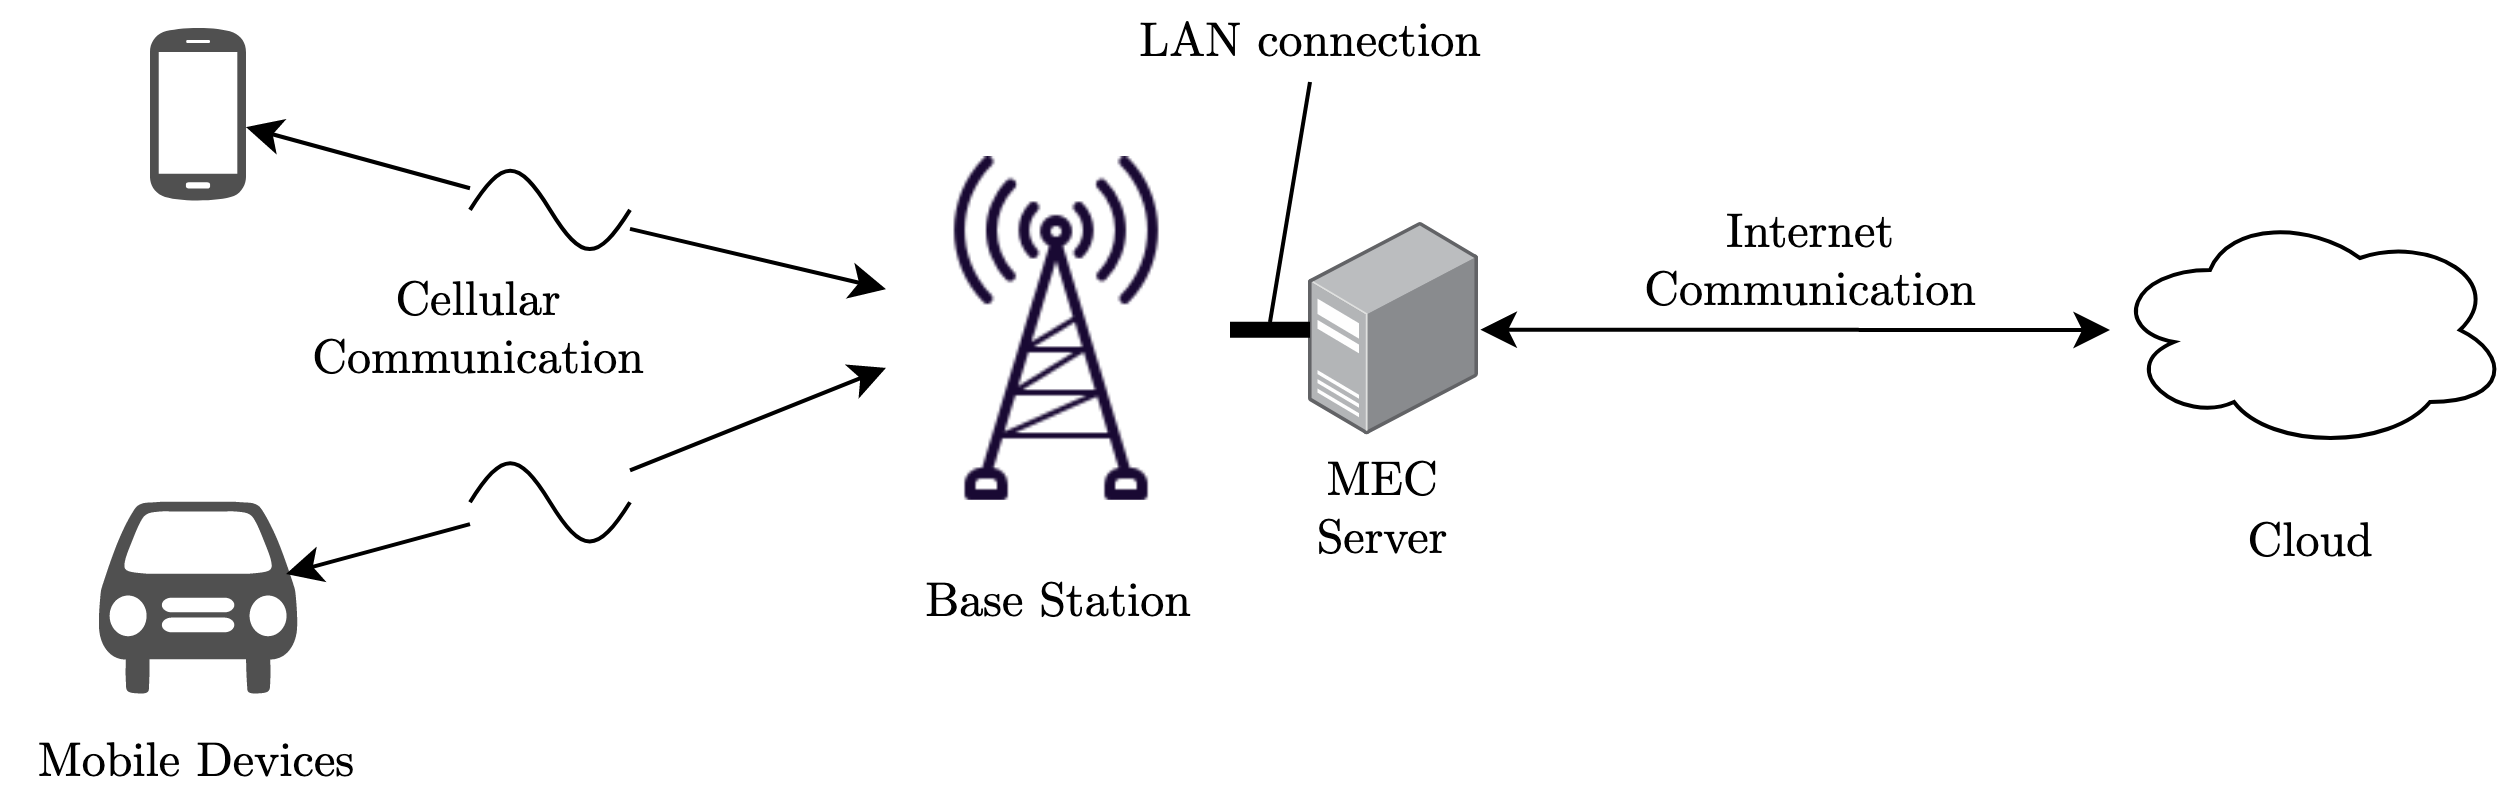
\includegraphics[scale=0.75]{chapters/architectures/figures/MEC.png}
    \caption{Diagram of MEC}
    \label{fig:MEC}
\end{figure}

Figure \ref{fig:MEC} shows how MEC works on a high level. MEC will utilize the ubiquitous cellular network to offload its work. At the base station there will be a MEC server that can provide storage and computational power to the mobile devices. However, the base station servers is not as powerful as the distant cloud servers. Since the base station is just one hop away, we don't have to necessarily deal with the dynamic internet. Additionally, the cellular network provides a very small delay, as base stations are relatively close by to almost everywhere where there are developed civilization. If the servers at the base station are overloaded they can send the work further to the really thick clients of the distant cloud or a CDN. The mobile devices can be any type of device that need storage offloading. The only requirement for this architecture is that it has a cellular connection.

The MEC server architecture is divided into several layers that together forms three systems\cite{patel_mec_nodate}. At the bottom is the hardware layer. Over that is the virtualization layer. These two layers is part of the MEC Hosting Infrastructure Management System. Over that is the MEC Application Platform Management System which consists of a MEC virtualization manager layer and and MEC Application Platform Services layer. The virtualization manager can provide IaaS. The MEC Application Platform Services layer is essentially an interface for the virtual machines that the applications is running on. The VMs and the apps form the Application Management Systems.
%TODO lag en figur her

% In our experiments, the Emerald VM will consist of the two bottom systems, and we will focus on the application layer.

%SDN er at vi har virtuelle nettverk. Slik som at vi har eget nettverk i AWS på jobben. Vi kan da definere virtuelle nettverksdrivere og interfaces osv. For eksempel ha et eget virtuellt nettverk til kun databaseting.
%NFV handler om at man kan ha virtuelle funksjoner på hver ruter feks. slik at man ikke trenger å sende pakker helt i datasentere. Du lar heller en aksess punkt eller cloudlet ta seg av funksjonen. Jeg ser for meg at det ligner AWS Lambda, bare at det heller kjører på en aksess punkt


% sjekk ut 22?, 122,121?, 161, 163
% 162!! NFV (Network Function Virtualization)
% 166 SDN(software defined networking og NFV )
% 175, 176 ICN(Information centric networking)
% 164 NFV MEC architecture for video, gaming and AR


\section{Cloudlet} \label{cloudlet} 
Satyanarayanan et al., proposed in their paper “The Case for VM-Based Cloudlets in Mobile Computing”\cite{satyanarayanan_case_2009} a solution to resource poverty of mobile devices and for the long latency in the Wide-Area Network(WAN). They raise the issue that humans will not tolerate significant delays when using applications. E.g. using a remote photo editing software. It does not matter how good the bandwidth is, the latency will hurt the interactive performance. Since WAN latency is unlikely to improve, we should rather move the thick client closer to the thin client. 

The proposed solution to this is Cloudlets, which are nearby resource-rich thick-clients. Since they are nearby they are one-hop, high bandwidth, low latency wirelessly accessible computers. The goal is to do all significant computation on a nearby cloudlet instead of doing so on the cell phone. Since the cloudlet is near and resource rich, you can get fast and predictable results, when you offload the work to it. Offloading helps the device get results faster, and use less power. A Cloudlet is essentially a data center in a box. To let different devices use it seamlessly, it uses VM’s that runs on top of the OS. A device can send a specification of a VM to the Cloudlet, and let it spin up. It also allows for migration of the VM, as we can expect the mobile device to move closer to another Cloudlet.


% Husk at cloudlet kan videre overføre til distant cloud.


\section{Content Delivery Networks}
Content Delivery Networks(CDN) are providers that have focused on putting servers close to the users. Firms like Akamai will have deals with local Internet Service Providers (ISP) to have some servers at their facilities. This ensures that their servers are only a few hops away from the clients. You also have technologies like Google AMP, which lets you have cached stripped down versions of websites cached at these CDNs to help speed up website loading.


%% bare skriv om en av de fog computing arkitekturene så er du i gang! :D


% TODO:

% Odessa
% MAUI

% peer to peer?

% MCC vs MEC
